\documentclass[letterpaper,12pt,fleqn]{article}
\usepackage{matharticle}
\usepackage{tikz}
\pagestyle{empty}
\begin{document}
\section*{Binomial Theorem}
\begin{theorem}
$\binom{n-1}{k}+\binom{n-1}{k-1}=\binom{n}{k}$
\end{theorem}
\begin{theproof}
\listbreak
\begin{enumerate}
\item{Analytical}
\begin{eqnarray*}
\binom{n-1}{k}+\binom{n-1}{k-1} &=& \frac{(n-1)!}{k!(n-1-k)!}+
  \frac{(n-1)!}{(k-1)![(n-1)-(k-1)]!} \\
    &=& \frac{(n-1)!}{k!(n-k-1)!}+\frac{(n-1)!}{(k-1)!(n-k)!} \\
    &=& \frac{(n-1)!(n-k)}{k!(n-k)!}+\frac{(n-1)!k}{k!(n-k)!} \\
    &=& \frac{(n-1)![(n-k)+k]}{k!(n-k)!} \\
    &=& \frac{(n-1)!n}{k!(n-k)!} \\
    &=& \frac{n!}{k!(n-k)!} \\
    &=& \binom{n}{k} \\
\end{eqnarray*}

\item{Combinatorial\vspace{0.25in} \\}
Consider the selection of a committee of size $k$ from a pool of $n$ people.
The RHS is the number of ways to select such a committee: $\binom{n}{k}$ ways.
For the LHS, select a particular person A and partition the selection process
into committees without A and committees with A.  For a committee without A,
all $k$ members must be selected from the remaining $n-1$ members, or
$\binom{n-1}{k}$ ways. For a committee with A, the remaining $k-1$ members must
be selected from the remaining $n-1$ members, or $\binom{n-1}{k-1}$ ways.
Therefore:
\[\binom{n-1}{k}+\binom{n-1}{k-1}=\binom{n}{k}\]

\item{Block-walking\vspace{0.25in} \\}
\begin{tikzpicture}
\draw [fill=black] (0,1) circle [radius=0.1];
\draw [fill=black] (1,0) circle [radius=0.1];
\draw [fill=black] (2,1) circle [radius=0.1];
\draw (0,1) -- (1,0) -- (2,1);
\node [above] at (0,1) {$\binom{n-1}{k-1}$};
\node [above] at (2,1) {$\binom{n-1}{k}$};
\node [below] at (1,0) {$\binom{n}{k}$};
\end{tikzpicture}
\end{enumerate}
\end{theproof}
\theoremstyle{mathitem}
\newtheorem*{binomial}{Binomial Theorem}
\begin{binomial}
$(a+b)^n=\sum_{k=0}^n\binom{n}{k}a^{n-k}b^k$
\end{binomial}
\begin{theproof}
By induction:
\subsubsection*{Base: n=1}
\[(a+b)^1=a+b\]
\begin{eqnarray*}
\sum_{k=0}^1\binom{n}{k}a^{n-k}b^k &=&
  \binom{1}{0}a^{1-0}b^0+\binom{1}{1}a^{1-1}b^1 \\
    &=& 1a^1b^0+1a^0b^1 \\
    &=& a+b \\
\end{eqnarray*}
\subsubsection*{Inductive Assumption}
Assume $(a+b)^n=\sum_{k=0}^n\binom{n}{k}a^{n-k}b^k$
\begin{eqnarray*}
(a+b)^{n+1} &=& (a+b)(a+b)^n \\
    &=& (a+b)\sum_{k=0}^n\binom{n}{k}a^{n-k}b^k \\
    &=& \sum_{k=0}^n\binom{n}{k}a^{n-k+1}b^k+\sum_{k=0}^n\binom{n}{k}a^{n-k}b^{k+1} \\
    &=& \sum_{k=0}^n\binom{n}{k}a^{n+1-k}b^k+
        \sum_{k=1}^{n+1}\binom{n}{k-1}a^{n-(k-1)}b^{(k-1)+1} \\
    &=& \sum_{k=0}^n\binom{n}{k}a^{n+1-k}b^k+
        \sum_{k=1}^{n+1}\binom{n}{k-1}a^{n+1-k}b^k \\
    &=& a^{n+1}+
        \sum_{k=1}^n\left[\binom{n}{k}+\binom{n}{k-1}\right]a^{n+1-k}b^k+
        b^{n+1} \\
    &=& a^{n+1}+\sum_{k=1}^n\binom{n+1}{k}a^{n+1-k}b^k+b^{n+1} \\
    &=& \sum_{k=0}^{n+1}\binom{n+1}{k}a^{(n+1)-k}b^k \\
\end{eqnarray*}
\end{theproof}
\end{document}
